\section{Preliminary Results}
\label{sec:results}

\subsection{Overall Retrieval Effectiveness}
Table~\ref{tab:main} summarizes retrieval performance across all configurations and tiers. 
At the two-stage reranking tier, \lineH\ achieves the highest aggregate effectiveness ($\text{NDCG@10} = 0.499$, 95\% CI $[0.450, 0.543]$), alongside the strongest Top-1 accuracy ($\text{NDCG@1} = 0.800$) and reciprocal rank ($\text{MRR@10} = 0.980$). 
\astH\ achieves $\text{NDCG@10} = 0.457$ ($[0.405, 0.509]$), followed by \lineN\ ($0.470$, $[0.414, 0.524]$) and \astN\ ($0.345$, $[0.299, 0.390]$).

Lexical BM25 scores low in all conditions (NDCG@10 between $0.104$ and $0.187$ across the four BM25 configurations in the package; Table~\ref{tab:main} lists the two with headers). 
Because BM25 was not used for pooling, most of its top-10 items are unjudged (Judged@10 $13.6\%$--$30.4\%$ across the four configurations) and count as zero; we therefore also report bpref, which ignores unjudged items~\cite{buckley2004bpref}. 
BM25 remains lowest (bpref $0.152$--$0.241$ across configurations) but the gap to the dense ($0.278$--$0.350$) and reranking tiers ($0.285$--$0.356$) is smaller than NDCG@10 suggests. 
BM25 still serves only as a reference, not as an unpenalized baseline. 
With headers, dense retrieval improves NDCG@10 over BM25 by $0.238$ to $0.322$, and reranking adds a further $0.048$ to $0.049$. 
Notably, context headers benefit AST chunks already at the dense bi-encoder tier ($\Delta = +0.088$, rising from $0.320$ to $0.408$) as well as during reranking ($\Delta = +0.112$, reaching $0.457$), confirming that headers serve as essential anchors during initial candidate retrieval. 
For the dense and reranking systems, Judged@3 is 100\% and Judged@10 is 53.6\% to 59.2\%.

\begin{table}[t]
\caption{Retrieval effectiveness ($N=25$ JDs). Rerank tier first; Dense and BM25 are reference tiers.}
\label{tab:main}
\centering\footnotesize
\setlength{\tabcolsep}{3pt}
\begin{threeparttable}
\begin{tabular}{@{}llcccc@{}}
\toprule
Chunk & Header & NDCG@10 [95\% CI] & NDCG@1 & MRR@10 & J@10\tnote{a} \\
\midrule
Line & Yes & \textbf{0.499} [0.450, 0.543] & \textbf{0.800} & \textbf{0.980} & 0.552 \\
Line & No  & \textit{0.470} [0.414, 0.524] & \textit{0.740} & 0.933 & 0.564 \\
AST  & Yes & 0.457 [0.405, 0.509] & 0.720 & \textit{0.940} & 0.564 \\
AST  & No  & 0.345 [0.299, 0.390] & 0.460 & 0.846 & 0.536 \\
\midrule
\multicolumn{6}{l}{\textit{Reference Tiers (Line+Header / AST+Header)}} \\
Dense & Yes (Line) & 0.450 [0.398, 0.502] & 0.580 & 0.913 & 0.572 \\
Dense & Yes (AST)  & 0.408 [0.346, 0.463] & 0.660 & 0.900 & 0.544 \\
BM25$^{\dagger}$ & Yes (Line) & 0.129 [0.094, 0.165] & 0.140 & 0.405 & 0.180 \\
BM25$^{\dagger}$ & Yes (AST)  & 0.170 [0.122, 0.221] & 0.080 & 0.395 & 0.244 \\
\bottomrule
\end{tabular}
\begin{tablenotes}\footnotesize
\item[] Bold: best; italic: second best within the reranking tier.
\item[a] Judged@10: share of top-10 items with a human label (unjudged count as 0).
\item[$\dagger$] BM25 was not used for pooling; scores are not an unpenalized baseline.
\end{tablenotes}
\end{threeparttable}
\end{table}


\subsection{Hypothesis Testing and Confirmatory Analyses}
Table~\ref{tab:statistical_hypothesis_tests} presents the statistical test results for the confirmatory family and the exploratory contrast.

\begin{figure}[t]
\centering
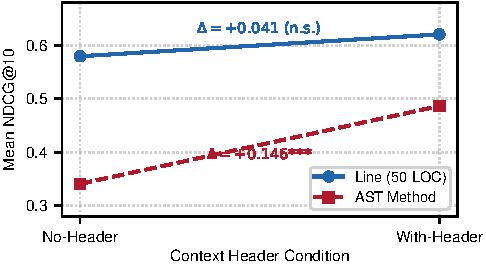
\includegraphics[width=0.88\columnwidth]{figs/fig1.pdf}
\caption{Interaction plot demonstrating differential context header sensitivity between line-window chunking and AST-first chunking at the reranking tier ($N=25$ JDs).}
\label{fig:interaction_plot}
\end{figure}

\begin{table}[t]
\caption{Hypothesis tests for the confirmatory family and the exploratory contrast (NDCG@10, rerank tier).}
\label{tab:statistical_hypothesis_tests}
\centering\footnotesize
\resizebox{\columnwidth}{!}{%
\begin{tabular}{@{}llccc@{}}
\toprule
ID & Contrast ($A - B$) & $\Delta$ [95\% CI] & W/L/T & $p_{\mathrm{Holm}}$ \\
\midrule
\multicolumn{5}{@{}l}{\emph{Confirmatory family (step-down Holm, $\alpha = 0.05$)}} \\
Comp 1 & \astH\ vs. \lineN & $-0.014$ [$-0.088$, $+0.058$] & 12/13/0 & 0.8532 \\
Comp 2 & \astN\ vs. \lineN & $-0.126$ [$-0.180$, $-0.076$] & 5/20/0  & $<0.001^{***}$ \\
Comp 3 & \astH\ vs. \astN  & $+0.112$ [$+0.056$, $+0.166$] & 19/6/0  & 0.0031$^{**}$ \\
Comp 4 & \lineH\ vs. \lineN & $+0.029$ [$-0.017$, $+0.078$] & 15/10/0 & 0.7332 \\
\midrule
\multicolumn{5}{@{}l}{\emph{Exploratory (outside the Holm family)}} \\
Comp 5 & \astH\ vs. \lineH & $-0.043$ [$-0.106$, $+0.021$] & 6/18/1  & 0.1355$^{\dagger}$ \\
\bottomrule
\end{tabular}%
}

\vspace{2pt}
\parbox{\columnwidth}{\footnotesize Significance follows $p_{\mathrm{Holm}}$ (** $<0.01$, *** $<0.001$). $^{\dagger}$Unadjusted $p_{\mathrm{raw}}$.}
\end{table}


\textbf{RQ1: Context Header Impact (Comps 3 and 4).}
Adding hierarchical context headers produces a statistically significant improvement for AST chunks (\textbf{Comp 3}: $\Delta = +0.112$, 95\% CI $[+0.056, +0.166]$, $p_{\mathrm{Holm}} = 0.0031$, $W = 46.0$). 
\astH\ outperforms \astN\ on 19 of the 25 JDs. 
In contrast, prepending context headers to line windows yields a small gain that we cannot distinguish from zero (\textbf{Comp 4}: $\Delta = +0.029$, 95\% CI [$-0.017$, $+0.078$], $p_{\mathrm{Holm}} = 0.7332$, $W = 128.0$; 15 wins vs. 10 losses). 
As shown in Fig.~\ref{fig:interaction_plot}, context headers act as an essential anchor for AST chunks while providing marginal benefits for line windows.

\textbf{RQ2: AST vs. Line-Window Chunking (Comps 1, 2, and 5).}
Comparing \astH\ against \lineN\ reveals no evidence of a difference (\textbf{Comp 1}: $\Delta = -0.014$, 95\% CI [$-0.088$, $+0.058$], $p_{\mathrm{Holm}} = 0.8532$, $W = 155.0$), with an even win/loss balance (12 vs. 13). 
Without headers (\textbf{Comp 2}), line windows outperformed AST chunks ($\Delta = -0.126$, 95\% CI [$-0.180$, $-0.076$], $p_{\mathrm{Holm}} = 0.0001$, $W = 22.0$), winning 20 of 25 queries. 
In the exploratory contrast with headers (\textbf{Comp 5}), line windows remain numerically higher ($\Delta = -0.043$, 95\% CI [$-0.106$, $+0.021$], $p_{\mathrm{raw}} = 0.1355$, $W = 97.0$; Line wins 18, AST wins 6, 1 tie), though the difference is not significant.

\subsection{Language Sensitivity and Fallback Audit}
Subgroup analysis across target ecosystems reveals marked divergence:
On Java repositories ($N=15$ JDs), \astH\ closely tracks \lineH\ ($\text{NDCG@10} = 0.515$ vs. $0.536$, $\Delta = -0.021$). 
On React/TypeScript repositories ($N=10$ JDs), the deficit widens more than threefold ($\text{NDCG@10} = 0.369$ vs. $0.445$, $\Delta = -0.075$).

The audit offers a possible mechanism: $35.7\%$ of AST-arm chunks (130/364) triggered the line-window fallback. 
Java had a low fallback rate ($13.1\%$, 20/153), driven by DTO/entity classes without methods (9), interface contracts (8), top-level classes/configurations (2), and records/enums (1). 
React/TypeScript had a $52.1\%$ fallback rate (110/211), caused by top-level JSX renders or non-method components (51), styled-components (23), object literals (13), TypeScript types (10), exported constant arrays (5), \texttt{forwardRef} wrappers (4), export defaults (3), and Redux slices (1). 
The largest React category may reflect gaps in our parser rather than inherently non-method code; refining it is part of the plan. 
In the top-10 retrieved results for the AST arm, fallback chunks constitute $70.0\%$ (175/250) of results without headers and $46.0\%$ (115/250) with headers.
